% defer/hazptr.tex
% From an C++ Standards Committee meeting:  "Can I hazptr cheezeberger?"

\section{Hazard Pointers}
\label{sec:defer:Hazard Pointers}
%
\epigraph{If in doubt, turn it inside out.}{\emph{Zara Carpenter}}

One way of avoiding problems with concurrent reference counting
is to implement the reference counters
inside out, that is, rather than incrementing an integer stored in the
data element, instead store a pointer to that data element in
per-CPU (or per-thread) lists.
Each element of these lists is called a
\emph{hazard pointer}~\cite{MagedMichael04a}.\footnote{
	Also independently invented by others~\cite{HerlihyLM02}.}
The value of a given data element's ``virtual reference counter'' can
then be obtained by counting the number of hazard pointers referencing
that element.
Therefore, if that element has been rendered inaccessible to readers,
and there are no longer any hazard pointers referencing it, that element
may safely be freed.

\begin{listing}[tbp]
\input{CodeSamples/defer/hazptr@record_clear.fcv}
\caption{Hazard-Pointer Recording and Clearing}
\label{lst:defer:Hazard-Pointer Recording and Clearing}
\end{listing}

Of course, this means that hazard-pointer acquisition must be carried
out quite carefully in order to avoid destructive races with concurrent
deletion.
\begin{lineref}[ln:defer:hazptr:record_clear]
One implementation is shown in
Listing~\ref{lst:defer:Hazard-Pointer Recording and Clearing},
which shows \co{hp_try_record()} on lines~\lnref{htr:b}-\lnref{htr:e},
\co{hp_record()} on lines~\lnref{hr:b}-\lnref{hr:e}, and
\co{hp_clear()} on
lines~\lnref{hc:b}-\lnref{hc:e} (\path{hazptr.h}).

The \co{hp_try_record()} macro on line~\lnref{htr:e} is simply a casting
wrapper for the \co{_h_t_r_impl()} function, which attempts to store
the pointer referenced by \co{p} into the hazard pointer referenced
by \co{hp}.
If successful, it returns the value of the stored pointer.
If it fails due to that pointer being \co{NULL}, it returns \co{NULL}.
Finally, if it fails due to racing with an update, it returns a special
\co{HAZPTR_POISON} token.

\QuickQuiz{}
	Given that papers on hazard pointers use the bottom bits
	of each pointer to mark deleted elements, what is up with
	\co{HAZPTR_POISON}?
\QuickQuizAnswer{
	The published implementations of hazard pointers used
	non-blocking synchronization techniques for insertion
	and deletion.
	These techniques require that readers traversing the
	data structure ``help'' updaters complete their updates,
	which in turn means that readers need to look at the successor
	of a deleted element.

	In contrast, we will be using locking to synchronize updates,
	which does away with the need for readers to help updaters
	complete their updates, which in turn allows us to leave
	pointers' bottom bits alone.
	This approach allows read-side code to be simpler and faster.
} \QuickQuizEnd

Line~\lnref{htr:ro1} reads the pointer to the object to be protected.
If line~\lnref{htr:race1} finds that this pointer was either \co{NULL} or
the special \co{HAZPTR_POISON} deleted-object token, it returns
the pointer's value to inform the caller of the failure.
Otherwise, line~\lnref{htr:store} stores the pointer into the specified
hazard pointer, and line~\lnref{htr:mb} forces full ordering of that
store with the reload of the original pointer on line~\lnref{htr:ro2}.
(See Chapter~\ref{chp:Advanced Synchronization: Memory Ordering}
for more information on memory ordering.)
If the value of the original pointer has not changed, then the hazard
pointer protects the pointed-to object, and in that case,
line~\lnref{htr:success} returns a pointer to that object, which also
indicates success to the caller.
Otherwise, if the pointer changed between the two \co{READ_ONCE()}
invocations, line~\lnref{htr:race2} indicates failure.

\QuickQuiz{}
	Why does \co{hp_try_record()} in
	Listing~\ref{lst:defer:Hazard-Pointer Recording and Clearing}
	take a double indirection to the data element?
	Why not \co{void *} instead of \co{void **}?
\QuickQuizAnswer{
	Because \co{hp_try_record()} must check for concurrent modifications.
	To do that job, it needs a pointer to a pointer to the element,
	so that it can check for a modification to the pointer to the
	element.
} \QuickQuizEnd

The \co{hp_record()} function is quite straightforward: It repeatedly
invokes \co{hp_try_record()} until the return value is something other
than \co{HAZPTR_POISON}.

\QuickQuiz{}
	Why bother with \co{hp_try_record()}?
	Wouldn't it be easier to just use the failure-immune
	\co{hp_record()} function?
\QuickQuizAnswer{
	It might be easier in some sense, but as will be seen in the
	Pre-BSD routing example, there are situations for which
	\co{hp_record()} simply does not work.
} \QuickQuizEnd

The \co{hp_clear()} function is even more straightforward, with
an \co{smp_mb()} to force full ordering between the caller's uses
of the object protected by the hazard pointer and the setting of
the hazard pointer to \co{NULL}.
\end{lineref}

\begin{listing}[tbp]
\input{CodeSamples/defer/hazptr@scan_free.fcv}
\caption{Hazard-Pointer Scanning and Freeing}
\label{lst:defer:Hazard-Pointer Scanning and Freeing}
\end{listing}

\begin{lineref}[ln:defer:hazptr:scan_free:free]
Once a hazard-pointer-protected object has been removed from its
linked data structure, so that it is now inaccessible to future
hazard-pointer readers, it is passed to \co{hazptr_free_later()},
which is shown on lines~\lnref{b}-\lnref{e} of
Listing~\ref{lst:defer:Hazard-Pointer Scanning and Freeing}
(\path{hazptr.c}).
Lines~\lnref{enq:b} and~\lnref{enq:e}
enqueue the object on a per-thread list \co{rlist}
and line~\lnref{count} counts the object in \co{rcount}.
If line~\lnref{check} sees that a sufficiently large number of objects are now
queued, line~\lnref{scan} invokes \co{hazptr_scan()} to attempt to
free some of them.
\end{lineref}

\begin{lineref}[ln:defer:hazptr:scan_free:scan]
The \co{hazptr_scan()} function is shown on lines~\lnref{b}-\lnref{e}
of the listing.
This function relies on a fixed maximum number of threads (\co{NR_THREADS})
and a fixed maximum number of hazard pointers per thread (\co{K}),
which allows a fixed-size array of hazard pointers to be used.
Because any thread might need to scan the hazard pointers, each thread
maintains its own array, which is referenced by the per-thread variable
\co{gplist}.
If line~\lnref{check} determines that this thread has not yet allocated its
\co{gplist}, lines~\lnref{alloc:b}-\lnref{alloc:e} carry out the allocation.
The memory barrier on line~\lnref{mb1} ensures that all threads see the
removal of all objects by this thread before
lines~\lnref{loop:b}-\lnref{loop:e} scan
all of the hazard pointers, accumulating non-NULL pointers into
the \co{plist} array and counting them in \co{psize}.
The memory barrier on line~\lnref{mb2} ensures that the reads of
the hazard pointers
happen before any objects are freed.
Line~\lnref{sort} then sorts this array to enable use of binary search below.

Lines~\lnref{rem:b} and~\lnref{rem:e}
remove all elements from this thread's list of
to-be-freed objects, placing them on the local \co{tmplist}
and line~\lnref{zero} zeroes the count.
Each pass through the loop spanning
lines~\lnref{loop2:b}-\lnref{loop2:e} processes each
of the to-be-freed objects.
Lines~\lnref{rem1st:b} and~\lnref{rem1st:e}
remove the first object from \co{tmplist},
and if lines~\lnref{chkhazp:b} and~\lnref{chkhazp:e}
determine that there is a hazard pointer
protecting this object, lines~\lnref{back:b}-\lnref{back:e}
place it back onto \co{rlist}.
Otherwise, line~\lnref{free} frees the object.
\end{lineref}

\begin{listing}[tbp]
\input{CodeSamples/defer/route_hazptr@lookup.fcv}
\caption{Hazard-Pointer Pre-BSD Routing Table Lookup}
\label{lst:defer:Hazard-Pointer Pre-BSD Routing Table Lookup}
\end{listing}

The Pre-BSD routing example can use hazard pointers as shown in
Listing~\ref{lst:defer:Hazard-Pointer Pre-BSD Routing Table Lookup}
for data structures and \co{route_lookup()}, and in
Listing~\ref{lst:defer:Hazard-Pointer Pre-BSD Routing Table Add/Delete}
for \co{route_add()} and \co{route_del()}
(\path{route_hazptr.c}).
As with reference counting, the hazard-pointers implementation
is quite similar to the sequential algorithm shown in
Listing~\ref{lst:defer:Sequential Pre-BSD Routing Table}
on
page~\pageref{lst:defer:Sequential Pre-BSD Routing Table},
so only differences will be discussed.

\begin{lineref}[ln:defer:route_hazptr:lookup]
Starting with
Listing~\ref{lst:defer:Hazard-Pointer Pre-BSD Routing Table Lookup},
line~\lnref{hh} shows the \co{->hh} field used to queue objects pending
hazard-pointer free,
line~\lnref{re_freed} shows the \co{->re_freed} field used to detect
use-after-free bugs, and line~\lnref{tryrecord} invokes
\co{hp_try_record()} to attempt to acquire a hazard pointer.
If the return value is \co{NULL}, line~\lnref{NULL} returns a not-found
indication to the caller.
If the call to \co{hp_try_record()} raced with deletion, line~\lnref{deleted}
branches back to line~\lnref{retry}'s \co{retry} to re-traverse the list
from the beginning.
The \co{do}-\co{while} loop falls through when the desired element is
located, but if this element has already been freed, line~\lnref{abort}
terminates the program.
Otherwise, the element's \co{->iface} field is returned to the caller.

Note that line~\lnref{tryrecord} invokes \co{hp_try_record()} rather
than the easier-to-use \co{hp_record()}, restarting the full search
upon \co{hp_try_record()} failure.
And such restarting is absolutely required for correctness.  To see this,
consider a hazard-pointer-protected linked list containing elements~A,
B, and~C that is subjected to the following sequence of events:
\end{lineref}

\begin{enumerate}
\item	Thread~0 stores a hazard pointer to element~B
	(having presumably traversed to element~B from element~A).
\item	Thread~1 removes element~B from the list, which sets
	the pointer from element~B to element~C to the special
	\co{HAZPTR_POISON} value in order to mark the deletion.
	Because Thread~0 has a hazard pointer to element~B,
	it cannot yet be freed.
\item	Thread~1 removes element~C from the list.
	Because there are no hazard pointers referencing element~C,
	it is immediately freed.
\item	Thread~0 attempts to acquire a hazard pointer to now-removed
	element~B's successor, but \co{hp_try_record()} returns the
	\co{HAZPTR_POISON} value, forcing the caller to restart its
	traversal from the beginning of the list.
\end{enumerate}

Which is a very good thing, because B's successor is the now-freed
element~C, which means that Thread~0's subsequent accesses might have
resulted in arbitrarily horrible memory corruption, especially if the
memory for element~C had since been re-allocated for some other purpose.
Therefore, hazard-pointer readers must typically restart the full
traversal in the face of a concurrent deletion.
Often the restart must go back to some global (and thus immortal) pointer,
but it is sometimes possible to restart at some intermediate location
if that location is guaranteed to still be live, for example, due to
the current thread holding a lock, a reference count, etc.

\QuickQuiz{}
	Readers must ``typically'' restart?
	What are some exceptions?
\QuickQuizAnswer{
	If the pointer emanates from a global variable or is otherwise
	not subject to being freed, then \co{hp_record()} may be
	used to repeatedly attempt to record the hazard pointer,
	even in the face of concurrent deletions.
	% @@@ Add more use cases subject to Maged Michael's approval.
} \QuickQuizEnd

Because algorithms using hazard pointers might be restarted at any
step of their traversal through the linked data structure, such algorithms
must typically take care to avoid making any changes to the data
structure until after they have acquired all the hazard pointers that
are required for the update in question.

\QuickQuiz{}
	But don't these restrictions on hazard pointers also apply
	to other forms of reference counting?
\QuickQuizAnswer{
	Yes and no.
	These restrictions apply only to reference-counting mechanisms whose
	reference acquisition can fail.
} \QuickQuizEnd

These hazard-pointer restrictions result in great benefits to readers,
courtesy of the fact that the hazard pointers are stored local to each
CPU or thread, which in turn allows traversals to be carried out without
any writes to the data structures being traversed.
Referring back to
Figure~\ref{fig:count:Optimization and the Four Parallel-Programming Tasks}
on
page~\pageref{fig:count:Optimization and the Four Parallel-Programming Tasks},
hazard pointers enable the CPU caches to do resource replication, which
in turn allows weakening of the parallel-access-control mechanism,
thus boosting performance and scalability.

Another advantage of hazard pointers's restarting is a reduction in its
minimal memory footprint:
Any object not currently referenced by some hazard pointer may be
immediately freed.
In contrast,
Section~\ref{sec:defer:Read-Copy Update (RCU)}
will discuss a mechanism that avoids read-side retries (and minimizes
read-side overhead), but which can result in a much larger memory
footprint.

\begin{listing}[tbp]
\input{CodeSamples/defer/route_hazptr@add_del.fcv}
\caption{Hazard-Pointer Pre-BSD Routing Table Add\slash Delete}
\label{lst:defer:Hazard-Pointer Pre-BSD Routing Table Add/Delete}
\end{listing}

\begin{lineref}[ln:defer:route_hazptr:add_del]
In
Listing~\ref{lst:defer:Hazard-Pointer Pre-BSD Routing Table Add/Delete},
line~\lnref{init_freed} initializes \co{->re_freed},
line~\lnref{poison} poisons the \co{->re_next} field of the newly removed
object, and
line~\lnref{free_later} passes that object to the hazard pointers's
\co{hazptr_free_later()} function, which will free that object once it
is safe to do so.
The spinlocks work the same as in
Listing~\ref{lst:defer:Reference-Counted Pre-BSD Routing Table Add/Delete}.
\end{lineref}

\begin{figure}[tb]
\centering
\resizebox{2.5in}{!}{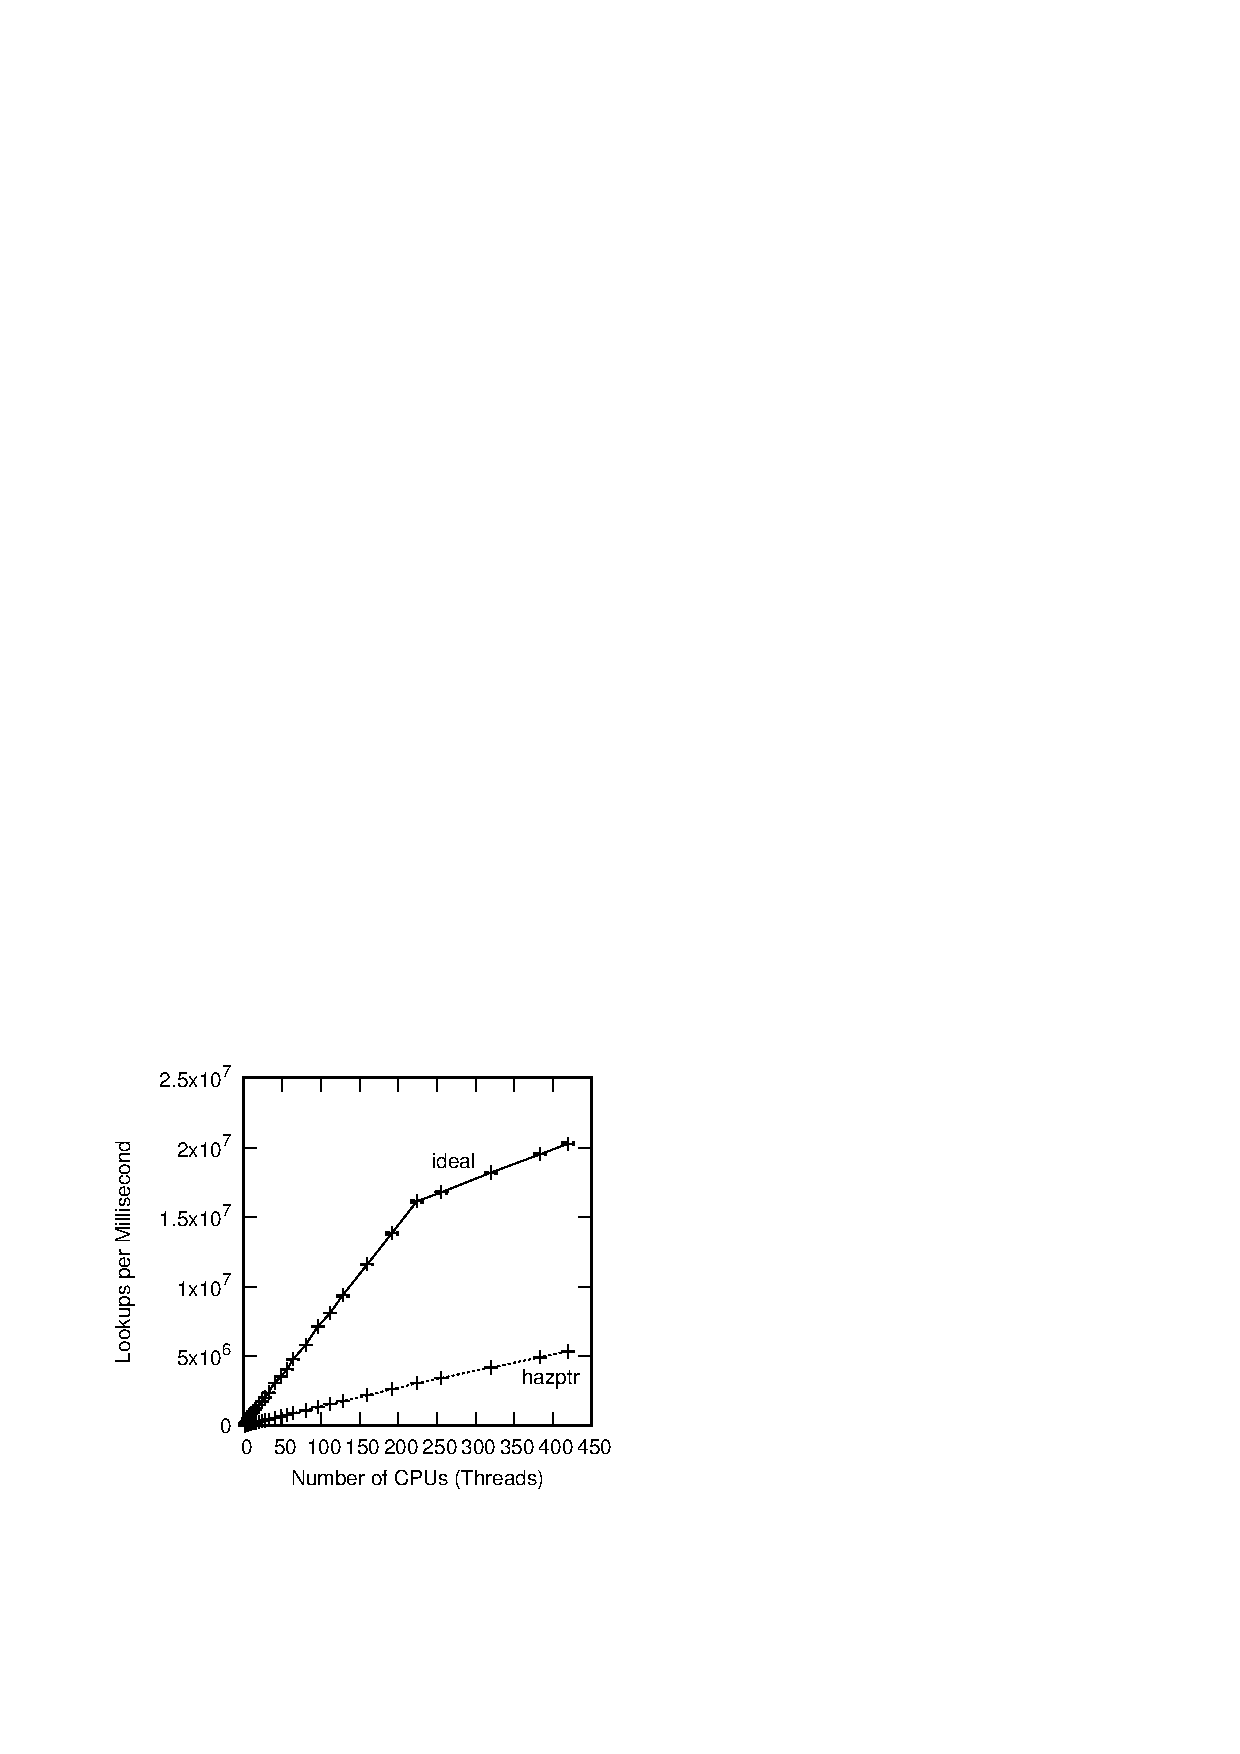
\includegraphics{CodeSamples/defer/perf-hazptr}}
\caption{Pre-BSD Routing Table Protected by Hazard Pointers}
\label{fig:defer:Pre-BSD Routing Table Protected by Hazard Pointers}
\end{figure}

Figure~\ref{fig:defer:Pre-BSD Routing Table Protected by Hazard Pointers}
shows the hazard-pointers-protected Pre-BSD routing algorithm's
performance on the same read-only workload as for
Figure~\ref{fig:defer:Pre-BSD Routing Table Protected by Reference Counting}.
Although hazard pointers scales much better than does reference counting,
hazard pointers still require readers to do writes to shared
memory (albeit with much improved locality of reference),
and also require a full memory barrier and retry check for each
object traversed.
Therefore, hazard pointers's performance is far short of ideal.
On the other hand, unlike naive approaches to concurrent reference-counting,
hazard pointers do operate correctly for workloads
involving concurrent updates.
Additional performance comparisons with other mechanisms may be found in
Chapter~\ref{chp:Data Structures}
and in other publications~\cite{ThomasEHart2007a,McKenney:2013:SDS:2483852.2483867,MagedMichael04a}.

\QuickQuiz{}
	The paper ``Structured Deferral: Synchronization via
	Procrastination''~\cite{McKenney:2013:SDS:2483852.2483867}
	shows that hazard pointers have near-ideal performance.
	Whatever happened in
	Figure~\ref{fig:defer:Pre-BSD Routing Table Protected by Hazard Pointers}???
\QuickQuizAnswer{
	First,
	Figure~\ref{fig:defer:Pre-BSD Routing Table Protected by Hazard Pointers}
	has a linear y-axis, while most of the graphs in the
	``Structured Deferral'' paper have logscale y-axes.
	Next, that paper uses lightly-loaded hash tables, while
	Figure~\ref{fig:defer:Pre-BSD Routing Table Protected by Hazard Pointers}'s
	uses a 10-element simple linked list, which means that hazard pointers
	face a larger memory-barrier penalty in this workload than in
	that of the ``Structured Deferral'' paper.
	Finally, that paper used a larger and older x86 system, while
	a newer but smaller system was used to generate the data
	shown in
	Figure~\ref{fig:defer:Pre-BSD Routing Table Protected by Hazard Pointers}.

	In addition, use of pairwise asymmetric
	barriers~\cite{Windows2008FlushProcessWriteBuffers,JonathanCorbet2010sys-membarrier,Linuxmanpage2018sys-membarrier}
	has been proposed to eliminate the read-side hazard-pointer
	memory barriers on systems supporting this notion~\cite{DavidGoldblatt2018asymmetricFences},
	which might improve the performance of hazard pointers beyond
	what is shown in the figure.

	As always, your mileage may vary.
	Given the difference in performance, it is clear that hazard
	pointers give you the most ideal performance either for
	very large data structures (where the memory-barrier overhead
	will at least partially overlap cache-miss penalties) and
	for data structures such as hash tables where a lookup
	operation needs a minimal number of hazard pointers.
} \QuickQuizEnd

The next section attempts to improve on hazard pointers by using
sequence locks, which avoid both read-side writes and per-object memory
barriers.
